\documentclass[a4paper,twoside]{article}
\usepackage[T1]{fontenc}
\usepackage[bahasa]{babel}
\usepackage{color} %warna
\usepackage{graphicx}
\usepackage{graphics}
\usepackage{float}
\usepackage[cm]{fullpage}
\pagestyle{myheadings}
\usepackage{etoolbox}
\usepackage{setspace} 
\usepackage{lipsum} 
\usepackage{listings} %source code
\usepackage{lscape} %landscape untuk source code
\usepackage{multicol} %multiple column
\usepackage{ifthen} % if then
\setlength{\headsep}{30pt}
\usepackage[inner=2cm,outer=2.5cm,top=2.5cm,bottom=2cm]{geometry} %margin
% \pagestyle{empty}
\usepackage{url}

\makeatletter
\renewcommand{\@maketitle} {\begin{center} {\LARGE \textbf{ \textsc{\@title}} \par} \bigskip {\large \textbf{\textsc{\@author}} }\end{center} }
\renewcommand{\thispagestyle}[1]{}
\markright{\textbf{\textsc{Laporan Perkembangan Pengerjaan Skripsi\textemdash Sem. Ganjil 2015/2016}}}

\onehalfspacing
 
\begin{document}

\title{\@judultopik}
\author{\nama \textendash \@npm} 

%ISILAH DATA DATA BERIKUT INI:
\newcommand{\nama}{Tommy Adhitya The}
\newcommand{\@npm}{2012730031}
\newcommand{\tanggal}{11/10/2015} %Tanggal pembuatan dokumen
\newcommand{\@judultopik}{\textit{Porting} PHP menjadi Java/Play Framework (Studi Kasus KIRI \textit{Dashboard Server Side})} % Judul/topik anda
\newcommand{\kodetopik}{PAS3901}
\newcommand{\jumpemb}{1} % Jumlah pembimbing, 1 atau 2
\newcommand{\pembA}{Pascal Alfadian, M.Com.}
\newcommand{\pembB}{-}
\newcommand{\semesterPertama}{39 - Ganjil 15/16} % semester pertama kali topik diambil, angka 1 dimulai dari sem Ganjil 96/97
\newcommand{\lamaSkripsi}{1} % Jumlah semester untuk mengerjakan skripsi s.d. dokumen ini dibuat
\newcommand{\kulPertama}{Skripsi 1} % Kuliah dimana topik ini diambil pertama kali
\newcommand{\tipePR}{B} % tipe progress report :
% A : dokumen pendukung untuk pengambilan ke-2 di Skripsi 1
% B : dokumen untuk reviewer pada presentasi dan review Skripsi 1
% C : dokumen pendukung untuk pengambilan ke-2 di Skripsi 2
\maketitle

\pagenumbering{arabic}

\lstset{
  numbers=left,
  stepnumber=1,    
  firstnumber=1,
  numberfirstline=true
}
\lstset{basicstyle=\tiny, commentstyle=\color{blue}}
\lstset{frame=leftline, tabsize=4, breaklines=true}

\section{Data Skripsi} %TIDAK PERLU MENGUBAH BAGIAN INI !!!
Pembimbing utama/tunggal: {\bf \pembA}\\
Pembimbing pendamping: {\bf \pembB}\\
Kode Topik : {\bf \kodetopik}\\
Topik ini sudah dikerjakan selama : {\bf \lamaSkripsi} semester\\
Pengambilan pertama kali topik ini pada : Semester {\bf \semesterPertama} \\
Pengambilan pertama kali topik ini di kuliah : {\bf \kulPertama} \\
Tipe Laporan : {\bf \tipePR} -
\ifdefstring{\tipePR}{A}{
			Dokumen pendukung untuk {\BF pengambilan ke-2 di Skripsi 1} }
		{
		\ifdefstring{\tipePR}{B} {
				Dokumen untuk reviewer pada presentasi dan {\bf review Skripsi 1}}
			{	Dokumen pendukung untuk {\bf pengambilan ke-2 di Skripsi 2}}
		}

\section{Detail Perkembangan Pengerjaan Skripsi}
Detail bagian pekerjaan skripsi sesuai dengan rencan kerja/laporan perkembangan terkahir :
	\begin{enumerate}
		\item Mempelajari kode situs web KIRI \textit{Dashboard Server Side}(bahasa PHP).\\
		{\bf status :} Ada sejak rencana kerja skripsi.\\
		{\bf hasil :}
		
		Berikut adalah kode situs web KIRI \textit{Dashboard Server Side}(bahasa PHP):
\begin{lstlisting}[language=PHP,basicstyle=\tiny,caption=handle.php,label={lst:handle.php}]
<?php
require_once '../../etc/utils.php';
require_once '../../etc/constants.php';
require_once '../../etc/PasswordHash.php';

start_working();

$mode = retrieve_from_post($proto_mode);

// Initializes MySQL and check for session
init_mysql();
if ($mode != $proto_mode_login && $mode != $proto_mode_logout && $mode != $proto_mode_register) {
	$sessionid = addslashes(retrieve_from_post($proto_sessionid));
	// Clear expired sessions
	mysqli_query($global_mysqli_link, "DELETE FROM sessions WHERE lastSeen < (NOW() - INTERVAL $session_expiry_interval_mysql)") or
		die_nice('Failed to clean expired sessions: ' . mysqli_error($global_mysqli_link), true);
	$result = mysqli_query($global_mysqli_link, "SELECT users.email, users.privilegeRoute, users.privilegeApiUsage FROM users LEFT JOIN sessions ON users.email = sessions.email WHERE sessions.sessionId = '$sessionid'") or
		die_nice('Failed to get user session information: ' . mysqli_error($global_mysqli_link), true);
	if (mysqli_num_rows($result) == 0) {
		deinit_mysql();
		// Construct json - session expired.
		$json = array(
			$proto_status => $proto_status_sessionexpired,
		);
		print(json_encode($json));
		exit(0);
	}
	$columns = mysqli_fetch_row($result);
	$active_userid = $columns[0]; 
	$privilege_route = $columns[1] != '0';
	$privilege_apiUsage = $columns[2] != '0';
}

if ($mode == $proto_mode_login) {
	$userid = addslashes(retrieve_from_post($proto_userid));
	$plain_password = addslashes(retrieve_from_post($proto_password));
	if (strlen($userid) > $maximum_userid_length) {
		return_invalid_credentials("User ID length is more than allowed (". strlen($userid) . ')');
	}
	if (strlen($plain_password) > $maximum_password_length) {
		return_invalid_credentials('Password length is more than allowed ('. strlen($password) . ')');
	}

	// Retrieve the user information
	$result = mysqli_query($global_mysqli_link, "SELECT * FROM users WHERE email='$userid'") or
		die_nice('Failed to verify user id: ' . mysqli_error($global_mysqli_link), true);
	if (mysqli_num_rows($result) == 0) {
		deinit_mysql();
		return_invalid_credentials("User id not found: $userid");
	}
	$userdata = mysqli_fetch_assoc($result);
	
	// Check against the stored hash.
	$hasher = new PasswordHash($passwordhash_cost_log2, $passwordhash_portable);
	if (!$hasher->CheckPassword($plain_password, $userdata['password'])) {
		log_statistic("$apikey_kiri", 'LOGIN', $userid . '/FAIL');
		deinit_mysql();
		return_invalid_credentials("Password mismatch for $userid");
	}
	
	log_statistic("$apikey_kiri", 'LOGIN', $userid . '/SUCCESS');
	
	// Create session id
	$sessionid = generate_sessionid();
	mysqli_query($global_mysqli_link, "INSERT INTO sessions (sessionId, email) VALUES ('$sessionid', '$userid')") or
		die_nice('Failed to generate session: ' . mysqli_error($global_mysqli_link), true);

	// Construct privilege lists
	$privileges = '';
	if ($userdata['privilegeRoute'] != 0) {
		$privileges .= ",$proto_privilege_route";
	}
	if ($userdata['privilegeApiUsage'] != 0) {
		$privileges .= ",$proto_privilege_apiUsage";
	}
	if (strlen($privileges) > 0) {
		$privileges = substr($privileges, 1);
	}
	
	// Construct json.
	$json = array(
			$proto_status => $proto_status_ok,
			$proto_sessionid => $sessionid,
			$proto_privileges => $privileges
	);
	
	deinit_mysql();
	print(json_encode($json));
} elseif ($mode == $proto_mode_logout) {
	$sessionid = addslashes(retrieve_from_post($proto_sessionid));

	// Remove the session information
	$result = mysqli_query($global_mysqli_link, "DELETE FROM sessions WHERE sessionId='$sessionid'") or
		die_nice('Failed to logout sessionid $sessionid: ' . mysqli_error($global_mysqli_link), true);
	deinit_mysql();
	well_done();	
} elseif ($mode == $proto_mode_add_track) {
	check_privilege($privilege_route); 
	$trackid = addslashes(retrieve_from_post($proto_trackid));
	$trackname = addslashes(retrieve_from_post($proto_trackname));
	$tracktype = addslashes(retrieve_from_post($proto_tracktype));
	$penalty = addslashes(retrieve_from_post($proto_penalty));
	$internalinfo = addslashes(retrieve_from_post($proto_internalinfo, false)) or $internalinfo = '';
	
	// Check if the id is already existed
	$result = mysqli_query($global_mysqli_link, "SELECT trackId FROM tracks WHERE trackId='$trackid'") or
		die_nice('Failed to check trackid existence: ' . mysqli_error($global_mysqli_link), true);
	if (mysqli_num_rows($result) == 0) {
		mysqli_query($global_mysqli_link, "INSERT INTO tracks (trackId, trackTypeId, trackName, penalty, internalInfo) VALUES ('$trackid','$tracktype','$trackname','$penalty','$internalinfo')") or
			die_nice('Failed to add a new track: ' . mysqli_error($global_mysqli_link), true);
		update_trackversion();
	} else {
		die_nice("The trackId '$trackid' already existed.", true);
	}
	deinit_mysql();
	well_done();
} elseif ($mode == $proto_mode_update_track) {
	check_privilege($privilege_route);
	$trackid = addslashes(retrieve_from_post($proto_trackid));
	$newtrackid = addslashes(retrieve_from_post($proto_new_trackid));
	$tracktype = addslashes(retrieve_from_post($proto_tracktype));
	$trackname = addslashes(retrieve_from_post($proto_trackname));
	$internalinfo = addslashes(retrieve_from_post($proto_internalinfo, false)) or $internalinfo = '';
	$pathloop = retrieve_from_post($proto_pathloop) == 'true' ? 1 : 0;
	$penalty = addslashes(retrieve_from_post($proto_penalty));
	$transfernodes = retrieve_from_post($proto_transfernodes, false);
	
	// When changed, check if the id is already existed
	if ($newtrackid != $trackid) {
		$result = mysqli_query($global_mysqli_link, "SELECT trackId FROM tracks WHERE trackId='$newtrackid'") or
			die_nice('Failed to check trackid existence: ' . mysqli_error($global_mysqli_link), true);
		if (mysqli_num_rows($result) != 0) {
			die_nice("The new trackId '$newtrackid' already existed.", true);
		}
	}
	mysqli_query($global_mysqli_link, "UPDATE tracks SET trackTypeId='$tracktype', trackId='$newtrackid', trackName='$trackname', internalInfo='$internalinfo', pathloop='$pathloop', penalty='$penalty' WHERE trackId='$trackid'") or
		die_nice('Failed to update the track: ' . mysqli_error($global_mysqli_link));
	if (!is_null($transfernodes)) {
		$transfernodes = addslashes($transfernodes);
		mysqli_query($global_mysqli_link, "UPDATE tracks SET transferNodes='$transfernodes'WHERE trackId='$trackid'") or
			die_nice('Failed to update the track: ' . mysqli_error($global_mysqli_link));
	}
	update_trackversion();
	deinit_mysql();
	well_done();
} elseif ($mode == $proto_mode_list_tracks) {
	check_privilege($privilege_route);
	// Retrieve track list from database
	$result = mysqli_query($global_mysqli_link, 'SELECT trackTypeId, trackId, trackName FROM tracks ORDER BY trackTypeId, trackId') or
		die('Cannot retrieve the track names from database');
	$track_list = array();	
	while ($row = mysqli_fetch_row($result)) {
		$track_list[] = array($row[1], htmlspecialchars($row[0] . '/' . $row[2]));
	}
	// Retrieve track types list result from database
	$result = mysqli_query($global_mysqli_link, 'SELECT trackTypeId, name FROM tracktypes ORDER BY trackTypeId') or
		die_nice('Cannot retrieve the track types from database');
	$tracktype_list = array();
	while ($row = mysqli_fetch_row($result)) {
		$tracktype_list[] = array($row[0], htmlspecialchars($row[1]));
	}
	
	// Construct json.
	$json = array(
		$proto_status => $proto_status_ok,
		$proto_trackslist => $track_list,
		$proto_tracktypeslist => $tracktype_list
	);
	
	deinit_mysql();
	print(json_encode($json));
} elseif ($mode == $proto_mode_getdetails_track) {
	check_privilege($privilege_route);
	$trackid = addslashes(retrieve_from_post($proto_trackid));

	// Retrieve result from database and construct in XML format
	$result = mysqli_query($global_mysqli_link, "SELECT trackTypeId, trackName, internalInfo, AsText(geodata), pathloop, penalty, transferNodes FROM tracks WHERE trackId='$trackid'") or
		die_nice("Can't retrieve the track details from database: " . mysqli_error($global_mysqli_link), true);
	$i = 0;
	$row = mysqli_fetch_row($result);
	if ($row == FALSE) {
		die_nice("Can't find track information for '$trackid'", true);
	}
	$geodata = lineStringToLatLngArray($row[3]);
	// Construct json.
	$json = array(
		$proto_status => $proto_status_ok,
		$proto_trackid => $trackid,
		$proto_tracktype => $row[0],
		$proto_trackname => $row[1],
		$proto_internalinfo => $row[2],
		$proto_geodata => $geodata,
		$proto_pathloop => ($row[4] > 0 ? true : false),
		$proto_penalty => doubleval($row[5]),
		$proto_transfernodes => is_null($row[6]) ? array('0-' . (count($geodata) - 1)) : split(',', $row[6]), 
	);
	
	deinit_mysql();
	print(json_encode($json));
} elseif ($mode == $proto_mode_cleargeodata) {
	check_privilege($privilege_route);
	$trackid = addslashes(retrieve_from_post($proto_trackid));
	
	mysqli_query($global_mysqli_link, "UPDATE tracks SET geodata=NULL, transferNodes=NULL WHERE trackId='$trackid'") or
		die_nice('Failed to clear the geodata: ' . mysqli_error($global_mysqli_link), true);
	
	deinit_mysql();
	well_done();
} elseif ($mode == $proto_mode_importkml) {
	check_privilege($privilege_route);
	$trackid = addslashes(retrieve_from_post($proto_trackid));
	// Import KML file into a geodata in database
	if ($_FILES[$proto_uploadedfile]['error'] != UPLOAD_ERR_OK) {
		die_nice("Server script is unable to retrieve the file, with PHP's UPLOAD_ERR_xxx code: " . $_FILES[$proto_uploadedfile]['error'], true);
	}
	if ($_FILES[$proto_uploadedfile]['size'] > $max_filesize) {
		die_nice("Uploaded file size is greater than maximum size allowed ($max_filesize)", true);
	}
	$file = fopen($_FILES[$proto_uploadedfile]['tmp_name'], "r") or die_nice('Unable to open uploaded file', true);
	$haystack = '';
	while ($line = fgets($file)) {
		$haystack .= trim($line);
	}
	$num_matches = preg_match_all("/<LineString>.*<coordinates>(.*)<\/coordinates>.*<\/LineString>/i", $haystack, $matches, PREG_PATTERN_ORDER);
	if ($num_matches != 1) {
		die_nice("The KML file must contain exactly one <coordinate> tag inside one <LineString> tag. But I found $num_matches occurences", true);
	}
	fclose($file);
	
	// Start constructing output
	$output = 'LINESTRING(';
	$points = preg_split('/\s+/', $matches[1][0]);
	for ($i = 0, $size = sizeof($points); $i < $size; $i++) {
		list($x, $y, $z) = preg_split('/\s*,\s*/', $points[$i]);
		if ($i > 0) {
			$output .= ',';
		}
		$output .= "$x $y";
	}
	$output .= ')';
	mysqli_query($global_mysqli_link, "UPDATE tracks SET geodata=GeomFromText('$output'), transferNodes=NULL WHERE trackId='$trackid'") or
		die_nice("Error updating the goedata: " . mysqli_error($global_mysqli_link), true);
	update_trackversion();
	deinit_mysql();
	well_done();
} elseif ($mode == $proto_mode_delete_track) {
	check_privilege($privilege_route);
	$trackid = addslashes(retrieve_from_post($proto_trackid));
	
	init_mysql();
	
	// Check if the id is already existed
	mysqli_query($global_mysqli_link, "DELETE FROM tracks WHERE trackId='$trackid'") or
		die_nice('Failed to delete track $trackid: ' . mysqli_error($global_mysqli_link), true);
	if (mysqli_affected_rows($global_mysqli_link) == 0) {
		die_nice("The track $trackid was not found in the database", true);
	}
	update_trackversion();
	deinit_mysql();
	well_done();	
} elseif ($mode == $proto_mode_list_apikeys) {
	check_privilege($privilege_apiUsage);
	// Retrieve api key list from database
	$result = mysqli_query($global_mysqli_link, "SELECT verifier, domainFilter, description FROM apikeys WHERE email='$active_userid' ORDER BY verifier") or
		die_nice('Cannot retrieve the API keys list from database: ' . mysqli_error($global_mysqli_link));
	$apikey_list = array();	
	while ($row = mysqli_fetch_row($result)) {
		$apikey_list[] = array($row[0], $row[1], $row[2]);
	}
	
	// Construct json.
	$json = array(
		$proto_status => $proto_status_ok,
		$proto_apikeys_list => $apikey_list,
	);
	
	deinit_mysql();
	print(json_encode($json));
} elseif ($mode == $proto_mode_add_apikey) {
	check_privilege($privilege_apiUsage);
	$domainfilter = addslashes(retrieve_from_post($proto_domainfilter));
	$description = addslashes(retrieve_from_post($proto_description));
	$apikey = generate_apikey();
	
	// Retrieve api key list from database
	$result = mysqli_query($global_mysqli_link, "INSERT INTO apikeys(verifier, email, domainFilter, description) VALUES('$apikey', '$active_userid', '$domainfilter', '$description')") or
		die_nice('Cannot insert a new api key: ' . mysqli_error($global_mysqli_link));

	log_statistic("$apikey_kiri", 'ADDAPIKEY', $userid . $apikey);
	
	// Construct json.
	$json = array(
			$proto_status => $proto_status_ok,
			$proto_verifier => $apikey,
	);
	
	deinit_mysql();
	print(json_encode($json));
} elseif ($mode == $proto_mode_update_apikey) {
	check_privilege($privilege_apiUsage);
	$apikey = addslashes(retrieve_from_post($proto_verifier));
	$domainfilter = addslashes(retrieve_from_post($proto_domainfilter));
	$description = addslashes(retrieve_from_post($proto_description));
	// Ensure that this user has access to the apikey
	$result = mysqli_query($global_mysqli_link, "SELECT email FROM apikeys WHERE verifier='apikey'") or
		die_nice('Cannot check API key owner: ' . mysqli_error($global_mysqli_link));
	while ($row = mysqli_fetch_row($result)) {
		if ($row[0] != $active_userid) {
			die_nice("User $active_userid does not have privilege to update API Key $apikey");
		}
	}
	mysqli_query($global_mysqli_link, "UPDATE apikeys SET domainFilter='$domainfilter', description='$description' WHERE verifier='$apikey'") or
		die_nice('Failed to update API Key: ' . mysqli_error($global_mysqli_link));
	
	deinit_mysql();
	well_done();
} elseif ($mode == $proto_mode_register) {
	$email = addslashes(retrieve_from_post($proto_userid));
	$fullname = addslashes(retrieve_from_post($proto_fullname));
	$company = addslashes(retrieve_from_post($proto_company));

	// Check if the email has already been registered.
	$result = mysqli_query($global_mysqli_link, "SELECT email FROM users WHERE email='$email'") or
		die_nice('Cannot check user id existence: ' . mysqli_error($global_mysqli_link));
	if (mysqli_num_rows($result) > 0) {
		die_nice("Ooops! Email $email has already registered. Please check your mailbox or contact hello@kiri.travel");
	}

	// Generate and send password
	$password = generate_password();
	$hasher = new PasswordHash($passwordhash_cost_log2, $passwordhash_portable);
	$passwordHash = $hasher->HashPassword($password); 
	mysqli_query($global_mysqli_link, "INSERT INTO users(email, password, privilegeApiUsage, fullName, company) VALUES('$email', '$passwordHash', 1, '$fullname', '$company')") or
		die_nice('Cannot add new user $email: ' . mysqli_error($global_mysqli_link));	
	sendPassword($email, $password, $fullname);

	log_statistic("$apikey_kiri", 'REGISTER', "$email/$fullname/$company");
	
	deinit_mysql();
	well_done();
} elseif ($mode == $proto_mode_getprofile) {
		$email = $active_userid;
	
		$result = mysqli_query($global_mysqli_link, "SELECT fullName, company FROM users WHERE email='$email'") or
			die_nice('Cannot retrieve user details: ' . mysqli_error($global_mysqli_link));
		if ($row = mysqli_fetch_row($result)) {
			$fullname = $row[0];
			$company = $row[1];
		} else {
			die_nice("User $email not found in database.");
		} 
	
		deinit_mysql();
		// Construct json.
		$json = array(
				$proto_status => $proto_status_ok,
				$proto_fullname => $fullname,
				$proto_company => $company
		);
		
		print(json_encode($json));
} elseif ($mode == $proto_mode_update_profile) {
	$email = $active_userid;
	$password = addslashes(retrieve_from_post($proto_password, false));
	$fullname = addslashes(retrieve_from_post($proto_fullname));
	$company = addslashes(retrieve_from_post($proto_company));

	// Updates password if necessary
	if (!is_null($password) && $password != "") {		
		$hasher = new PasswordHash($passwordhash_cost_log2, $passwordhash_portable);
		$passwordHash = $hasher->HashPassword($password);
		mysqli_query($global_mysqli_link, "UPDATE users SET password='$passwordHash' WHERE email='$email'") or
			die_nice('Cannot update password for $email: ' . mysqli_error($global_mysqli_link));
	}
	mysqli_query($global_mysqli_link, "UPDATE users SET fullName='$fullname', company='$company' WHERE email='$email'") or
		die_nice('Cannot update profile for $email: ' . mysqli_error($global_mysqli_link));

	deinit_mysql();
	well_done();
} else {
	die_nice("Mode not understood: \"" . $mode . "\"", true);
}

/**
 * Return invalid credential error, close mysql connection, and exit.
 * @param string $logmessage the message to record in the log file.
 */
function return_invalid_credentials($logmessage) {
	global $proto_status, $proto_status_credentialfail, $errorlog_file, $global_mysqli_link;
	$ip_address = $_SERVER['REMOTE_ADDR'];
	log_error("Login failed (IP=$ip_address): $logmessage", '../' . $errorlog_file);
	$json = array(
		$proto_status => $proto_status_credentialfail);
	print(json_encode($json));
	mysqli_close($global_mysqli_link);
	exit(0);
}

/**
 * 
 * Simply checks the input parameter, when false do default action
 * to return "user does not have privilege"
 * @param boolean $privilege if false will return error
 */
function check_privilege($privilege) {
	if (!$privilege) {
		die_nice("User doesn't have enough privilege to perform the action.", true);
	}
}

/**
 * Scans a directory and remove files that have not been modified for max_age
 * @param string $path the path to the directory to clean 
 * @param int $max_age maximum age of the file in seconds
 * @return boolean true if okay, false if there's an error.
 */
function clean_temporary_files($path, $max_age) {
	$currenttime = time();
	if ($dirhandle = opendir($path)) {
		while (($file = readdir($dirhandle)) != FALSE) {
			$fullpath = "$path/$file";
			if (is_file($fullpath) && $currenttime - filemtime($fullpath) > $max_age) {
				if (!unlink($fullpath)) {
					return FALSE;
				}
			}
		}
		return TRUE;
	} else {
		return FALSE;
	}
}

?>
\end{lstlisting}

		Berdasarkan hasil analisa dan wawancara dengan kontributor kode, kode situs web KIRI \textit{Dashboard Server Side}(bahasa PHP) terbagi dalam 16 bagian yang masing-masing melayani sebuah permintaan tertentu.

\begin{itemize}
\item \textbf{Bagian Pemeriksaan \textit{Login}}

Bagian ini terletak di baris 12-32 dari ``handle.php'' (kode Listing \ref{lst:handle.php}). Bagian ini akan dieksekusi untuk semua ``\texttt{mode}'' pada permintaan POST kecuali ``\texttt{mode=login}'', ``\texttt{mode=logout}'', dan ``\texttt{mode=register}''. Bagian ini berfungsi untuk memeriksa apakah pengguna sudah melakukan \textit{login} terlebih dahulu untuk melakukan aksi-aksi tertentu.

Bagian ini diawali dengan memeriksa apakah pengguna memberikan \textit{session id} pada permintaan atau tidak (baris 13). Setelah itu, program akan membersihkan sesi-sesi di \textit{database} yang sudah kadaluwarsa (baris 14-16). Baris 17-18 memeriksa apakah \textit{session} yang dikirimkan dari permintaan masih \textit{valid} di \textit{database} atau tidak. Jika tidak, maka bagian ini akan mengembalikan respon yang menyatakan bahwa sesi tidak \textit{valid} dan permintaan tidak dapat dilanjutkan (baris 19-27). Jika \textit{valid}, maka bagian ini akan menginisialisasi beberapa variabel yang menampung \textit{privilege} dari pengguna yang aktif (baris 28-31).

\item \textbf{Bagian \textit{Login}}

Bagian ini terletak di baris 34-89 dari ``handle.php'' (kode Listing \ref{lst:handle.php}). Bagian ini akan dieksekusi hanya jika terdapat parameter ``\texttt{mode=login}'' pada permintaan POST. Bagian ini berfungsi untuk melakukan otentikasi pengguna terhadap \textit{server} KIRI \textit{Dashboard}. Bagian ini akan menentukan apakah pengguna memiliki hak akses terhadap KIRI \textit{Dashboard} apakah tidak.

Bagian ini diawali dengan memeriksa apakah pengguna mengirimkan \textit{userid} dan \textit{password} dengan ukuran yang sesuai apa tidak (baris 35-42). Setelah itu, program akan mengambil data informasi pengguna (berdasarkan \textit{userid}) ke \textit{database} sistem (baris 45-51). Bila data pengguna tidak ditemukan maka program akan mengembalikan pesan kesalahan (baris 49). Jika informasi pengguna ditemukan, maka selanjutnya \textit{password} yang dikirimkan pengguna akan dicek kecocokannya dengan \textit{password} yang tersimpan dalam \textit{database} (baris 54-55). Hasil kecocokan tersebut akan dicatat ke dalam data statistik \textit{server} (baris 56 atau 61). Bila \textit{password} cocok, maka server akan membangun sebuah \textit{session id} (baris 64-66) dan memberikan hak akses tertentu kepada pengguna (baris 68-78). Terakhir, \textit{server} akan membangun data JSON (baris 81-85) untuk dikirimkan ke pengguna (baris 88) sebagai pesan keberhasilan pengguna dalam melakukan otentikasi terhadap \textit{server}.

\item \textbf{Bagian \textit{Logout}}

Bagian ini terletak di baris 89-97 dari ``handle.php'' (kode Listing \ref{lst:handle.php}). Bagian ini akan dieksekusi hanya jika terdapat parameter ``\texttt{mode=logout}'' pada permintaan POST. Bagian ini berfungsi untuk menghentikan hubungan otentikasi dengan \textit{server} (menghilangkan hak akses). Hal tersebut bertujuan agar hak akses yang dimiliki pengguna tidak digunakan sembarangan oleh pengguna lain yang tidak berwenang.

Bagian ini diawali dengan memeriksa apakah pengguna memberikan \textit{session id} pada permintaan atau tidak (baris 90). Setelah itu, program akan membersihkan sesi-sesi (sesuai dengan \textit{session id} pengguna) yang terdapat dalam \textit{database} (baris 93-95). Terakhir, \textit{server} akan mengirimkan pesan dalam format JSON (baris 96) sebagai penanda bahwa pengguna berhasil melakukan \textit{logout}.

\item \textbf{Bagian Menambahkan Rute}

Bagian ini terletak di baris 97-117 dari ``handle.php'' (kode Listing \ref{lst:handle.php}). Bagian ini akan dieksekusi hanya jika terdapat parameter ``\texttt{mode=addtrack}'' pada permintaan POST. Bagian ini berfungsi untuk menambahkan sebuah rute jalan yang dapat ditempuh oleh kendaraan umum tertentu (contoh: angkot).

Bagian ini diawali dengan memeriksa apakah pengguna memiliki hak akses untuk menambahkan rute atau tidak (baris 98). Lalu memeriksa apakah pengguna mengirimkan data \textit{trackid}, \textit{trackname}, \textit{tracktype}, \textit{penalty}, dan \textit{internalinfo} pada permintaan atau tidak (baris 99-103). Setelah itu, program akan mengecek apakah rute jalan yang ingin ditambahkan pengguna sudah ada atau belum di \textit{database} (106-114). Bila rute jalan belum ada, maka rute jalan akan ditambahkan ke dalam \textit{database} (baris 109) dan \textit{server} akan mengirimkan pesan dalam format JSON (baris 116) sebagai penanda bahwa pengguna berhasil menambahkan rute jalan.

\item \textbf{Bagian Mengubah Rute}

Bagian ini terletak di baris 117-146 dari ``handle.php'' (kode Listing \ref{lst:handle.php}). Bagian ini akan dieksekusi hanya jika terdapat parameter ``\texttt{mode=updatetrack}'' pada permintaan POST. Bagian ini berfungsi untuk mengubah data sebuah rute jalan yang dapat ditempuh oleh kendaraan umum tertentu (contoh: angkot).

Bagian ini diawali dengan memeriksa apakah pengguna memiliki hak akses untuk mengubah rute atau tidak (baris 118). Lalu memeriksa apakah pengguna mengirimkan data \textit{trackid}, \textit{newtrackid}, \textit{trackname}, \textit{tracktype}, \textit{penalty}, \textit{pathloop}, \textit{transfernodes}  dan \textit{internalinfo} pada permintaan atau tidak (baris 119-126). Setelah itu, \textit{server} akan mengecek apakah rute yang ingin diubah pengguna sudah memenuhi aturan (\textit{trackid} harus sama dengan \textit{newtrackid}) atau tidak (129-143). Bila rute yang ingin diubah maka \textit{server} akan mengirimkan pesan dalam format JSON sebagai penanda bahwa pengguna berhasil mengubah rute rute jalan.

\item \textbf{Bagian Melihat Daftar Rute}

Bagian ini terletak di baris 146-172 dari ``handle.php'' (kode Listing \ref{lst:handle.php}). Bagian ini akan dieksekusi hanya jika terdapat parameter ``\texttt{mode=listtracks}'' pada permintaan POST. Bagian ini berfungsi untuk memberikan daftar rute jalan yang terdapat dalam \textit{database} sistem KIRI.

Bagian ini diawali dengan memeriksa apakah pengguna memiliki hak akses terhadap rute jalan atau tidak (baris 147). Setelah itu program akan mengambil data daftar rute jalan yang terdapat pada \textit{database} sistem KIRI (baris 149-154). Lalu program juga akan mengambil data daftar tipe rute jalan dari \textit{database} (baris 156-161). Data-data yang diperoleh program (rute jalan dan tipe rute jalan) akan diubah formatnya menjadi sebuah data JSON (baris 164-168). Terakhir, program akan mengirimkan data dalam format JSON tersebut ke pengguna (baris 171).

\item \textbf{Bagian Melihat Informasi Rute secara Detail}

Bagian ini terletak di baris 172-200 dari ``handle.php'' (kode Listing \ref{lst:handle.php}). Bagian ini akan dieksekusi hanya jika terdapat parameter ``\texttt{mode=getdetailstrack}'' pada permintaan POST. Bagian ini berfungsi untuk memberikan informasi detail tentang suatu rute jalan.

Bagian ini diawali dengan memeriksa apakah pengguna memiliki hak akses terhadap rute jalan atau tidak (baris 173). Lalu program akan memeriksa apakah pengguna memberikan \textit{trackid} pada permintaan atau tidak (baris 174). Selanjutnya program akan mengambil data dari \textit{database} sistem KIRI (baris 177-184). Data yang diperoleh dari \textit{database} tersebut akan diubah formatnya ke dalam format JSON (baris 186-196). Terakhir, program akan mengirimkan data dalam format JSON tersebut ke pengguna (baris 199).

\item \textbf{Bagian Menghapus Data Geografis suatu Rute}

Bagian ini terletak di baris 200-209 dari ``handle.php'' (kode Listing \ref{lst:handle.php}). Bagian ini akan dieksekusi hanya jika terdapat parameter ``\texttt{mode=cleargeodata}'' pada permintaan POST. Bagian ini berfungsi untuk menghapus data geografis suatu rute jalan yang terdapat dalam \textit{database} sistem KIRI.

Bagian ini diawali dengan memeriksa apakah pengguna memiliki hak akses terhadap rute jalan atau tidak (baris 201). Lalu program akan memeriksa apakah pengguna memberikan \textit{trackid} pada permintaan atau tidak (baris 202). Program akan langsung menghapus data geografis rute jalan sesuai dengan \textit{trackid} permintaan pengguna jika \textit{trackid} tersebut terdapat dalam \textit{database} sistem KIRI (baris 204-205). Terakhir, program akan mengirimkan pesan keberhasilan dalam format JSON kepada pengguna (baris 208).

\item \textbf{Bagian Impor Data KML}

Bagian ini terletak di baris 209-246 dari ``handle.php'' (kode Listing \ref{lst:handle.php}). Bagian ini akan dieksekusi hanya jika terdapat parameter ``\texttt{mode=importkml}'' pada permintaan POST. Bagian ini berfungsi untuk menambahkan data geografis suatu rute dimana data yang ditambahkan berasal dari sebuah \textit{file} dengan format KML (\textit{Keyhole Markup Language}). KML adalah format \textit{file} yang digunakan untuk menampilkan data geografis dalam aplikasi pemetaan\cite{kml}. 

Bagian ini diawali dengan memeriksa apakah pengguna memiliki hak akses terhadap rute jalan atau tidak (baris 210). Lalu program akan memeriksa apakah pengguna memberikan \textit{trackid} pada permintaan atau tidak (baris 211). Selanjutnya program akan memeriksa apakah \textit{file} pengguna memberikan \textit{file} dengan format sesuai atau tidak (baris 213-218). Pada baris 219-228 program akan mengambil data LineString yang terdapat pada \textit{file} dengan menggunakan \textit{regular expression} (baris 224). \textit{Regular expression} adalah karakter atau kata spesial yang digunakan untuk menjelaskan pola pencarian\cite{regex}. Baris 231-239 program akan membangun data LineString yang semula dalam format KML menjadi format WKT. Program akan menambahkan data LineString dalam WKT tersebut ke dalam \textit{database} sesuai dengan \textit{trackid} yang diberikan pengguna (baris 241-243). Terakhir, program akan mengirimkan pesan dalam format JSON sebagai penanda bahwa pengguna berhasil melakukan import data KML (baris 245).

\item \textbf{Bagian Menghapus Rute}

Bagian ini terletak di baris 246-261 dari ``handle.php'' (kode Listing \ref{lst:handle.php}). Bagian ini akan dieksekusi hanya jika terdapat parameter ``\texttt{mode=deletetrack}'' pada permintaan POST. Bagian ini berfungsi untuk menghapus suatu rute jalan yang terdapat dalam sistem KIRI.

Bagian ini diawali dengan memeriksa apakah pengguna memiliki hak akses terhadap rute jalan atau tidak (baris 247). Lalu program akan memeriksa apakah pengguna memberikan \textit{trackid} pada permintaan atau tidak (baris 248). Program akan memeriksa apakah terdapat {trackid} yang sesuai dengan {trackid} yang ada pada \textit{database} KIRI (baris 250-259). Bila terdapat \textit{trackid} yang sesuai, maka program akan menghapus rute jalan tersebut. Terakhir, program akan mengirimkan pesan keberhasilan dalam format JSON kepada pengguna (baris 260).

\item \textbf{Bagian Melihat Daftar API \textit{Keys}}

Bagian ini terletak di baris 261-279 dari ``handle.php'' (kode Listing \ref{lst:handle.php}). Bagian ini akan dieksekusi hanya jika terdapat parameter ``\texttt{mode=listapikeys}'' pada permintaan POST. Bagian ini berfungsi untuk memberikan daftar API \textit{keys} yang terdapat dalam database sistem KIRI.

Bagian ini diawali dengan memeriksa apakah pengguna memiliki hak akses terhadap penggunaan API atau tidak (baris 262). Setelah itu program akan mengambil data daftar API \textit{keys} yang terdapat pada \textit{database} sistem KIRI (baris 264-269). Data-data yang diperoleh program akan diubah formatnya menjadi sebuah data JSON (baris 272-275). Terakhir, program akan mengirimkan data dalam format JSON tersebut ke pengguna (baris 278).

\item \textbf{Bagian Menambahkan API \textit{Key}}

Bagian ini terletak di baris 279-299 dari ``handle.php'' (kode Listing \ref{lst:handle.php}). Bagian ini akan dieksekusi hanya jika terdapat parameter ``\texttt{mode=addapikey}'' pada permintaan POST. Bagian ini berfungsi untuk menambahkan sebuah data API \textit{key} ke dalam sistem KIRI.

Bagian ini diawali dengan memeriksa apakah pengguna memiliki hak akses terhadap API \textit{keys} atau tidak (baris 280). Lalu memeriksa apakah pengguna mengirimkan data \textit{domainfilter} dan \textit{description} pada permintaan atau tidak (baris 281-282). Setelah itu, program akan membangun sebuah API key secara acak (baris 283). Program akan menambahkan data API \textit{key} sesuai dengan data yang dikirimkan pengguna ke dalam \textit{database} KIRI (baris 286) dan mencatat proses penambahan tersebut ke dalam \textit{database} (baris 289). Terakhir, program akan membangun sebuah pesan keberhasilan dalam format JSON (baris 292-295) dan mengirimkan pesan tersebut kepada pengguna (baris 298).

\item \textbf{Bagian Mengubah API \textit{Key}}

Bagian ini terletak di baris 299-317 dari ``handle.php'' (kode Listing \ref{lst:handle.php}). Bagian ini akan dieksekusi hanya jika terdapat parameter ``\texttt{mode=updateapikey}'' pada permintaan POST. Bagian ini berfungsi untuk mengubah data sebuah API \textit{key} pada \textit{database} sistem KIRI.

Bagian ini diawali dengan memeriksa apakah pengguna memiliki hak akses terhadap API \textit{keys} atau tidak (baris 300). Lalu memeriksa apakah pengguna mengirimkan data \textit{apikey}, \textit{domainfilter}, dan \textit{description} pada permintaan atau tidak (baris 301-303). Setelah itu, program akan memeriksa apakah pengguna yang bersangkutan adalah pemilik API \textit{key} yang ingin diubah atau bukan (baris 305-311). Lalu program mengubah data API \textit{key} yang terdapat dalam database (baris 312) sesuai dengan permintaan pengguna. Terakhir, program akan mengirimkan pesan dalam format JSON sebagai penanda bahwa pengguna berhasil mengubah rute jalan.

\item \textbf{Bagian \textit{Register}}

Bagian ini terletak di baris 317-341 dari ``handle.php'' (kode Listing \ref{lst:handle.php}). Bagian ini akan dieksekusi hanya jika terdapat parameter ``\texttt{mode=register}'' pada permintaan POST. Bagian ini berfungsi untuk melakukan pendaftaran sebagai pengguna KIRI \textit{Dashboard}. Pendaftaran ini berguna agar pengguna bisa mendapatkan hak akses terhadap fitur-fitur yang terdapat dalam KIRI \textit{Dashboard}.

Bagian ini diawali dengan memeriksa apakah pengguna memberikan \textit{email}, \textit{fullname}, dan \textit{company} pada permintaan atau tidak (baris 318-320). Setelah itu, program akan memeriksa \textit{database} apakah data pengguna yang ingin dibuat sudah ada atau belum (baris 323-327). Bila belum ada, maka program akan membangun sebuah sandi secara acak untuk pengguna (baris 330-332). Program akan menambahkan data pengguna beserta sandi yang telah dibangun ke dalam \textit{database} sistem KIRI (baris 333). Sandi yang telah dibangun program juga dikirimkan ke alamat \textit{email} pengguna (baris 335). Lalu program mencatat proses tersebut ke dalam statistik \textit{database} sistem KIRI. Terakhir, program akan mengirimkan pesan dalam format JSON sebagai penanda bahwa pengguna berhasil melakukan proses registrasi (baris 340).

\item \textbf{Bagian Melihat Data Pribadi Pengguna}

Bagian ini terletak di baris 341-362 dari ``handle.php'' (kode Listing \ref{lst:handle.php}). Bagian ini akan dieksekusi hanya jika terdapat parameter ``\texttt{mode=getprofile}'' pada permintaan POST. Bagian ini berfungsi untuk memberikan informasi mengenai data pribadi pengguna.

Bagian ini diawali dengan memeriksa apakah data pengguna dengan \textit{email} yang dimiliki pengguna pada saat sesi tersebut ada atau tidak (baris 344-345). Jika data pengguna ditemukan maka program akan mengambil dan membangun data pengguna (baris 346-351). Data pengguna yang dibangun tersebut kemudian diubah ke dalam format JSON (baris 355-359). Terakhir, program mengirimkan data dalam format JSON yang telah dibangun kepada pengguna (baris 361).

\item \textbf{Bagian Mengubah Data Pribadi Pengguna}

Bagian ini terletak di baris 362-380 dari ``handle.php'' (kode Listing \ref{lst:handle.php}). Bagian ini akan dieksekusi hanya jika terdapat parameter ``\texttt{mode=updateprofile}'' pada permintaan POST. Bagian ini berfungsi untuk mengubah data pribadi pengguna yang sudah terdaftar dalam sistem KIRI.

Bagian ini diawali dengan memeriksa apakah pengguna memberikan \textit{password}, \textit{fullname}, dan \textit{company} pada permintaan atau tidak (baris 364-366). Bila pengguna memberikan \textit{password} dengan nilai \texttt{NULL} maka program akan membangun \textit{password} secara acak dan menambahkan \textit{password} tersebut ke dalam \textit{database} sistem KIRI sesuai dengan \textit{email} pengguna pada saat sesi tersebut (kode 369-374). Lalu program akan mengubah semua data pribadi pengguna sesuai dengan data yang diberikan oleh pengguna (baris 375-376). Terakhir, program mengirimkan pesan keberhasilan dalam format JSON kepada pengguna (baris 379).

\end{itemize}

		
		\item Melakukan studi literatur tentang MySQL Spatial Extensions, JDBC, Play Framework, dan JSON.\\
		{\bf status :} Ada sejak rencana kerja skripsi, kecuali JDBC, dan JSON\\
		{\bf hasil :}
		
		\begin{itemize}
			\item \textbf{MySQL Spatial Extensions}

	Suatu \textit{geographic feature}\cite{mysqlspatial} adalah sesuatu yang ada di bumi yang memiliki lokasi sebagai penunjuk letak keberadaannya. Geometri adalah cabang ilmu matematika yang digunakan untuk memodelkan suatu \textit{geographic feature}. Dengan geometri, suatu \textit{geographic feature} dapat dinyatakan sebagai sebuah titik, garis, ruang, ataupun bentuk lainnya. Suatu ``\textit{feature}'' yang dimaksud dalam istilah \textit{geographic feature} dapat berupa:
	\begin{enumerate}
		\item \textbf{\textit{An entity}}, contohnya adalah gunung, kolam, kota, dll.
		\item \textbf{\textit{A space}}, contohnya adalah daerah, cuaca, dll.
		\item \textbf{\textit{A definable location}}, contohnya adalah persimpangan jalan, yaitu suatu tempat khusus dimana terdapat 2 buah jalan yang saling berpotongan.
	\end{enumerate}
	
	MySQL adalah salah satu perangkat lunak yang digunakan untuk mengatur data-data (\textit{database}) suatu situs web. Bentuk MySQL adalah sekumpulan tabel yang umumnya memiliki hubungan antar satu dengan yang lainnya. Setiap tabel pada MySQL memiliki kolom dan baris. Kolom pada MySQL menyatakan daftar jenis baris yang ingin dibuat dan baris menyatakan banyaknya data yang ada dalam tabel.
	
	Penamaan suatu kolom dalam MySQL membutuhkan penentuan tipe data yang akan digunakan dalam kolom tersebut. Dalam MySQL terdapat tipe-tipe data yang umum digunakan seperti \textit{Varchar} untuk menyimpan karakter atau kata, \textit{Int} untuk menyimpan angka, \textit{Boolean} untuk menyimpan nilai ``\texttt{true}'' atau ``\texttt{false}'', dan tipe data lainnya. MySQL Spatial Extensions adalah perluasan dari tipe-tipe data yang disediakan MySQL untuk menyatakan nilai geometri dari suatu \textit{geographic feature}.
	
	Berdasarkan kemampuan penyimpanan nilai geometri, tipe data \textit{spatial} dapat dikelompokan ke dalam 2 jenis:
\begin{enumerate}
	\item Tipe data yang hanya dapat menyimpan sebuah nilai geometri saja, yaitu:
	\begin{itemize}
		\item \textbf{\textit{Geometry}}
		\item \textbf{\textit{Point}}
		\item \textbf{\textit{LineString}}
		\item \textbf{\textit{Polygon}}
	\end{itemize}
	\item Tipe data yang dapat menyimpan sekumpulan nilai geometri, yaitu:
	\begin{itemize}
		\item \textbf{\textit{MultiPoint}}
		\item \textbf{\textit{MultiLineString}}
		\item \textbf{\textit{MultiPolygon}}
		\item \textbf{\textit{GeometryCollection}}
	\end{itemize}
\end{enumerate}

\textbf{\textit{Point}}

\textit{Point} adalah nilai geometri yang merepresentasikan sebuah lokasi ke dalam suatu koordinat\cite{mysqlspatial}. Koordinat pada \textit{Point} terdiri dari nilai X dan Y dimana X merepresentasikan letak lokasi terhadap garis bujur dan Y merepresentasikan letak lokasi terhadap garis lintang. \textit{Point} tidak memiliki dimensi maupun nilai batasan. Contoh representasi \textit{Point} adalah Universitas Katolik Parahyangan direpresentasikan dalam koordinat X=107.6049079 dan Y=-6.874735 (gambar \ref{fig:2_UNPAR}).

\begin{figure}[htbp]
	\centering
		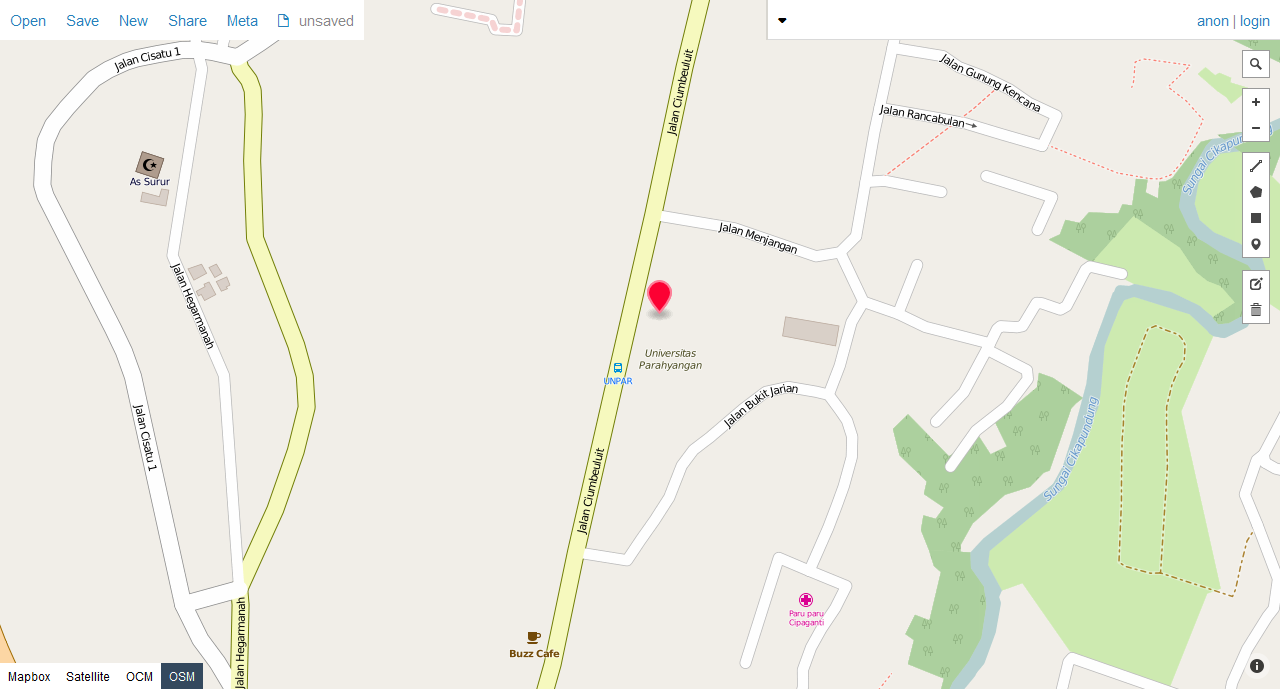
\includegraphics[scale=0.35]{Gambar/2_point.png}
	\caption{Universitas Katolik Parahyangan dinyatakan dalam \textit{Point}\cite{geojson}}
	\label{fig:2_UNPAR}
\end{figure}

\textbf{\textit{LineString}}

\textit{LineString} adalah garis yang terbentuk dari sekumpulan \textit{Point}\cite{mysqlspatial}. Dalam peta dunia, \textit{LineString} dapat merepresentasikan sebuah sungai dan dalam peta perkotaan, \textit{LineString} dapat merepresentasikan sebuah jalan (contoh: gambar \ref{fig:2_linestring}). Karena \textit{LineString} merupakan sekumpulan \textit{Point}, maka \textit{LineString} menyimpan sekumpulan koordinat dimana setiap koordinat ($X_{1}$\ldots$X_{n}$ dan $Y_{1}$\ldots$Y_{n}$, dimana n menyatakan banyaknya \textit{Point} dalam \textit{LineString}) terhubung oleh garis dengan koordinat selanjutnya. Contohnya: misal terdapat sebuah \textit{LineString} yang mengandung 3 buah \textit{Point}, maka terdapat garis yang menghubungkan \textit{Point} pertama dengan \textit{Point} kedua dan \textit{Point} kedua dengan \textit{Point} ketiga.

\begin{figure}[htbp]
	\centering
		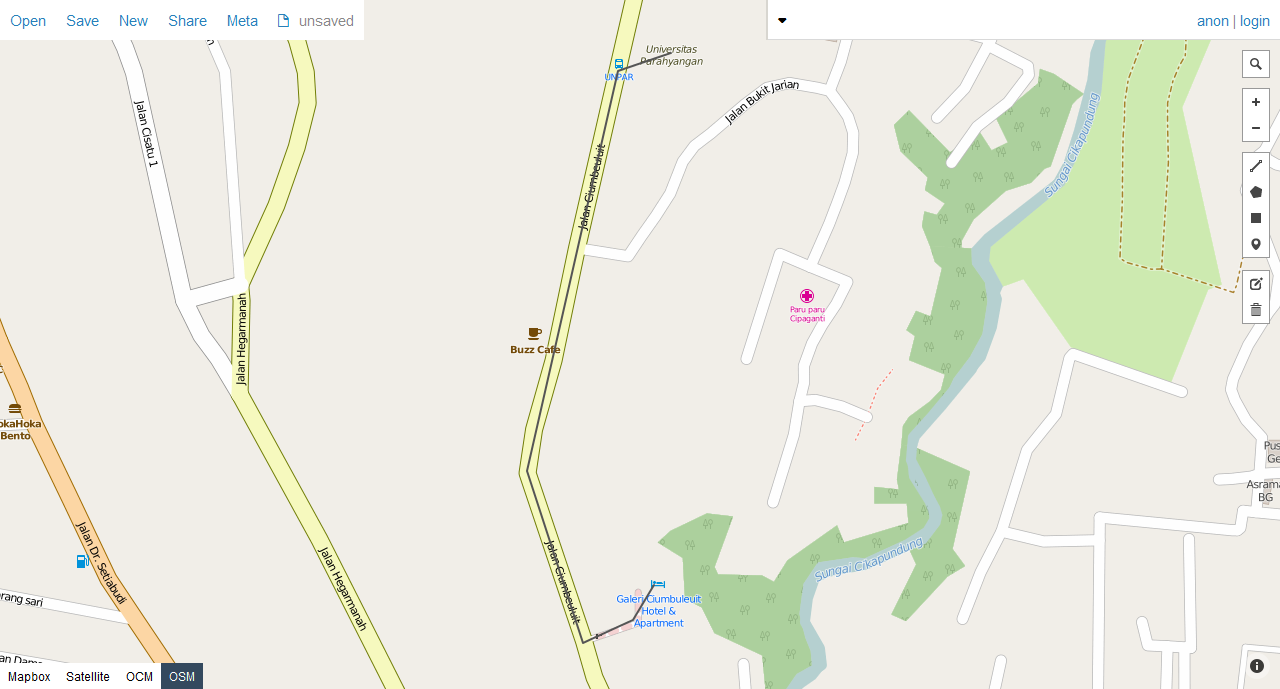
\includegraphics[scale=0.35]{Gambar/2_linestring.png}
	\caption{Rute jalan dari Universitas Katolik Parahyangan menuju Galeri Ciumbuleuit dinyatakan dalam \textit{LineString}\cite{geojson}}
	\label{fig:2_linestring}
\end{figure}

\textbf{Format Well-Known Text (WKT)}

Format Well-Known Text (WKT) adalah salah satu aturan penulisan tipe data \textit{spatial} untuk merepresentasikan suatu \textit{geographic feature}\cite{mysqlspatial}. WKT merepresentasikan nilai geometri yang dimodelkan untuk pertukaran data geometri dalam ASCII \textit{form}. Berikut adalah contoh format WKT:

\begin{lstlisting}
	POINT(107.6049079 -6.874735)
	
	LINESTRING(107.60502219200134 -6.875194997571583, 
						 107.60445356369019 -6.875386727913034,
						 107.60347723960876 -6.879647382202341,
						 107.6040780544281 -6.881479451795388,
						 107.60461449623108 -6.8812344661545986,
						 107.60483980178833 -6.880861661676069)
\end{lstlisting}

Contoh di atas menunjukkan format WKT dari \textit{Point} (baris 1) dan format WKT dari \textit{LineString} (baris 3-8).

Berikut adalah contoh penggunaan format WKT dalam MySQL:

\begin{lstlisting}
	CREATE TABLE geom (g LINESTRING);

	INSERT INTO geom VALUES (ST_GeomFromText('LINESTRING(107.60502219200134 -6.875194997571583, 
						 107.60445356369019 -6.875386727913034,
						 107.60347723960876 -6.879647382202341,
						 107.6040780544281 -6.881479451795388,
						 107.60461449623108 -6.8812344661545986,
						 107.60483980178833 -6.880861661676069)'));
	
	SELECT ST_AsText(g) FROM geom;
\end{lstlisting}

Contoh di atas menunjukkan pembuatan tabel ``\texttt{geom}'' dengan sebuah kolom ``\texttt{g}'' dan tipe data ``\texttt{LINESTRING}'' (baris 1), menambahkan 1 baris data berupa \textit{LineString} ke dalam tabel ``\texttt{geom}'' (baris 3-8), dan melihat data dari tabel ``\texttt{geom}'' (baris 10), dimana nilai kembalian ``\texttt{ST\_AsText(g)}'' berupa data \textit{LineString} dalam format WKT .



\item \textbf{JDBC}

JDBC API adalah bagian dari Java API yang dapat digunakan untuk mengakses semua jenis data yang terstruktur, terutama data yang tersimpan dalam suatu \textit{Relational Database}\cite{javadocumentation}. JDBC dapat membantu 3 jenis aktivitas \textit{programming} dalam menggunakan bahasa Java, yaitu:
\begin{enumerate}
	\item Menghubungkan aplikasi Java ke suatu sumber data seperti \textit{database},
	\item Mengirimkan \textit{queries} dan pembaharuan \textit{statement} ke \textit{database},
	\item Menerima dan melakukan proses terhadap hasil yang didapatkan dari pengiriman \textit{queries} tersebut.
\end{enumerate}
Berikut adalah contoh struktur kode yang mewakili 3 jenis aktivitas yang dapat dilakukan JDBC API:

\begin{lstlisting}
public void connectToAndQueryDatabase(String username, String password) {

    Connection con = DriverManager.getConnection(
                         "jdbc:myDriver:myDatabase",
                         username,
                         password);

    Statement stmt = con.createStatement();
    ResultSet rs = stmt.executeQuery("SELECT a, b, c FROM Table1");

    while (rs.next()) {
        int x = rs.getInt("a");
        String s = rs.getString("b");
        float f = rs.getFloat("c");
    }
}
\end{lstlisting}

Contoh di atas menunjukkan bagaimana JDBC API membantu aplikasi Java membuat koneksi terhadap suatu \textit{database} (baris 3-6), membuat dan mengirimkan suatu \textit{query} ke \textit{database} (baris 8 dan 9), dan menerima dan melakukan proses terhadap hasil yang didapatkan dari pengiriman \textit{query} tersebut (baris 9-15).

\textbf{\textit{Interface} Connection}

\textit{Interface} Connection adalah sebuah koneksi (\textit{session}) dengan \textit{database} spesifik\cite{javadocumentation}. Eksekusi SQL \textit{statements} dan penerimaan hasil kembalian dari eksekusi tersebut dapat terjadi karena adanya koneksi dengan \textit{database} yang dibentuk oleh \textit{interface} Connection. Berikut adalah sebagian \textit{method} yang ada pada \textit{interface} Connection:
\begin{itemize}
	\item \texttt{void close()}
	
	\textit{Method} ini digunakan untuk memutuskan koneksi dengan \textit{database} yang sedang terhubung.
	
	\item \texttt{Statement createStatement()}
	
	\textit{Method} ini digunakan untuk membangun objek \texttt{Statement} yang dapat digunakan untuk mengirimkan SQL \textit{statements} ke \textit{database} yang sedang terhubung.
\end{itemize}

\textbf{Kelas DriverManager}

Kelas DriverManager adalah cara paling dasar untuk mengatur JDBC \textit{drivers}\cite{javadocumentation}. Berikut adalah salah satu \textit{method} yang ada di kelas DriverManager untuk mengatur JDBC \textit{drivers}:
\begin{itemize}
	\item \texttt{public static Connection getConnection(String url, String user, String password)}
	
	\textit{Method} ini digunakan untuk membangun sebuah koneksi dengan \textit{database}. Umumnya method ini digunakan untuk membangun \textit{interface} Connection.
	
	Parameter:
	\begin{enumerate}
		\item \texttt{url}, alamat dari \textit{database}, formatnya adalah ``\textit{jdbc:\textit{subprotocol}:\textit{subname}}'',
		\item \texttt{user}, \textit{username} untuk mengakses \textit{database},
		\item \texttt{password}, \textit{password} dari \textit{username}.
	\end{enumerate}
	
	Nilai kembalian: sebuah koneksi terhadap \textit{database} yang sesuai dengan alamat \texttt{url}.
\end{itemize}

\textbf{\textit{Interface} Statement}

\textit{Interface} Statement adalah objek yang digunakan untuk melakukan eksekusi terhadap suatu \textit{query} dan mengembalikan nilai kembalian dari eksekusi tersebut\cite{javadocumentation}. Berikut adalah salah satu \textit{method} yang ada di \textit{interface} Statement:
\begin{itemize}
	\item \texttt{ResultSet executeQuery(String sql)}
	
	Parameter: \texttt{sql}, sebuah SQL \textit{statement} yang akan dikirimkan ke \textit{database}.
	
	Nilai kembalian: objek \texttt{ResultSet} yang berupa data yang dihasilkan dari eksekusi \textit{query} \texttt{sql}.
\end{itemize}

\textbf{\textit{Interface} ResultSet}

\textit{Interface} ResultSet adalah sebuah tabel data yang merepresentasikan hasil dari sebuah eksekusi \textit{query} pada suatu \textit{database}\cite{javadocumentation}. Cara kerja \textit{interface} ResultSet adalah dengan sistem indeks. Pada awalnya indeks ResultSet menunjuk pada data ``bayangan'' sebelum data pertama. Setiap pemanggilan \textit{method} ``\texttt{next()}'' pada objek ResultSet akan menyebabkan nilai indeks semakin meningkat (bertambah 1). Berikut adalah contoh \textit{method} \textit{interface} ResultSet:
\begin{itemize}
	\item \texttt{boolean next()}
	
	Nilai kembalian: \texttt{true} jika terdapat data pada indeks selanjutnya, \texttt{false} bila tidak ditemukan data pada indeks selanjutnya.

	\item \texttt{Object getObject(String columnLabel)}
	
	Parameter: \texttt{columnLabel}, merupakan nama kolom yang ingin diambil nilainya.
	
	Nilai kembalian: data berupa \texttt{Object} pada indeks baris dan kolom yang ditunjuk.
	
	\item \texttt{String getString(String columnLabel)}
	
	Parameter: \texttt{columnLabel}, merupakan nama kolom yang ingin diambil nilainya.
	
	Nilai kembalian: data berupa \texttt{String} pada indeks baris dan kolom yang ditunjuk.
	
	\item \texttt{int getInt(String columnLabel)}
	
	Parameter: \texttt{columnLabel}, merupakan nama kolom yang ingin diambil nilainya.
	
	Nilai kembalian: data berupa \texttt{int} pada indeks baris dan kolom yang ditunjuk.
	
	\item \texttt{boolean getBoolean(String columnLabel)}
	
	Parameter: \texttt{columnLabel}, merupakan nama kolom yang ingin diambil nilainya.
	
	Nilai kembalian: data berupa \texttt{boolean} pada indeks baris dan kolom yang ditunjuk.
\end{itemize}



\item \textbf{Play Framework}

Play Framework adalah sekumpulan kerangka kode yang dapat digunakan untuk membangun suatu situs web\cite{playforjava}. Play Framework tidak hanya menggunakan bahasa Java dalam pembuatannya. Bahasa Scala juga digunakan Play Framework dalam beberapa bagian seperti bagian \textit{view} dan \textit{route}. Play Framework menggunakan konsep MVC (\textit{Model} \textit{View} \textit{Controller}) sebagai pola arsitekturnya. Konsep MVC pada suatu kode membuat kode mudah dikembangkan baik secara tampilan maupun pengembangan fitur-fiturnya. Ketika \textit{server} Play Framework dijalankan, secara \textit{default} dapat diakses melalui ``localhost:9000''.

\textbf{Struktur Aplikasi}

Ketika Play Framework pertama kali ter-\textit{install} pada komputer, Play Framework menyediakan \textit{default} direktori dengan struktur minimal (gambar \ref{fig:2_strukturplay}). Berikut adalah penjelasan struktur minimal Play Framework:
\begin{enumerate}
	\item \textit{Folder} ``app'' merupakan \textit{folder} yang berisi mengenai pola arsitektur yang dimiliki Play Framework, yaitu ``models'' (tidak dibuat secara \textit{default}), ``views'', dan ``controllers''.
	\item \textit{Folder} ``conf'' berisi mengenai \textit{file} ``application.conf'' yang menyimpan pengaturan-pengaturan seperti kumpulan \textit{log}, koneksi ke \textit{database}, jenis \textit{port} tempat \textit{server} bekerja, dll. \textit{Folder} ``conf'' juga berisi \textit{file} ``routes'' yang mengatur bagaimana HTTP \textit{requests} nantinya akan diproses lebih lanjut.
	\item \textit{Folder} ``project'' terdapat \textit{file} ``build.properties'' dan ``plugins.sbt'', \textit{file} tersebut mendeskripsikan versi Play dan SBT yang digunakan pada aplikasi.
	\item \textit{Folder} ``public'' merupakan \textit{folder} yang menyimpan data-data seperti gambar (\textit{folder} ``images''), kumpulan Javascript yang digunakan (\textit{folder} ``javascripts'', secara \textit{default} berisikan \textit{file} ``jquery-1.9.0.min.js'') dan data-data CSS (folder ``stylesheets'').
	\item \textit{File} ``build.sbt'' mengatur \textit{dependencies} yang dibutuhkan dalam pembuatan aplikasi.
	\item Terakhir adalah \textit{folder} ``test'' yang merupakan salah satu kelebihan dari Play Framework, bagian ini berisikan \textit{file} ``Application.test'' dan ``Integration.test'' yang dapat digunakan untuk melakukan serangkaian \textit{testing} yang diinginkan terhadap aplikasi.
\end{enumerate}
     

\begin{figure}[htbp]
	\centering
		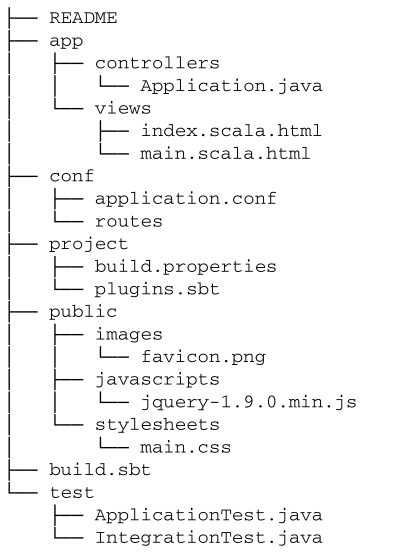
\includegraphics[scale=0.7]{Gambar/2_strukturplay.PNG}
	\caption{Struktur minimal Play Framework}
	\label{fig:2_strukturplay}
\end{figure}

\textbf{\textit{Routes}}

\textit{Routes} adalah \textit{file} yang mengatur pemetaan dari HTTP URLs menuju kode aplikasi (dalam hal ini menuju ke \textit{controllers}). Secara \textit{default}, \textit{routes} berisikan kode yang dapat memetakan permintaan URL \textit{index} standar seperti ``localhost:9000'' ketika \textit{server} Play Framework sudah dijalankan.

Berikut adalah isi kode \textit{default} \textit{routes}:

\begin{lstlisting}
	# Home page
	GET     /                           controllers.Application.index()

	# Map static resources from the /public folder to the /assets URL path
	GET     /assets/*file               controllers.Assets.at(path="/public", file)
\end{lstlisting}

Contoh di atas menunjukkan bagaimana \textit{routes} memetakan permintaan URL \textit{index} atau ``/'' (baris ke 2) dan permintaan URL ``/assets/*file'' (baris ke 5).

Struktur \textit{routes} terdiri dari 3 bagian (gambar \ref{fig:2_routes}), yaitu HTTP \textit{method}, URL \textit{path}, dan \textit{action method}. Struktur \textit{routes} seperti yang dijelaskan pada gambar \ref{fig:2_routes} juga sekaligus menjadi struktur minimal yang harus ada agar \textit{routes} dapat memetakan suatu HTTP URLs. HTTP \textit{method} berisikan protokol yang ingin dilakukan terhadap suatu HTTP \textit{request}. HTTP \textit{method} dapat berupa ``\texttt{GET}'', ``\texttt{POST}'', ``\texttt{DELETE}'', ``\texttt{PATCH}'', ``\texttt{HEAD}'' atau ``\texttt{PUT}''\cite{playframeworkweb}. URL \textit{path} merupakan direktori yang ingin dituju dalam \textit{server} aplikasi. URL \textit{path} dimulai dengan tanda ``/'' dan diikuti dengan nama direktori yang ingin dituju. Terakhir, \textit{action method} merupakan pemilihan kelas \textit{controller} yang ingin dituju. Struktur \textit{action method} terdiri dari 3 bagian (dipisahkan dengan karakter ``.''), yaitu pemilihan \textit{package} ``controllers'' yang ingin dituju, bagian kedua adalah pemilihan kelas ``controllers'' yang dipilih (contohnya: ``Products'' pada gambar \ref{fig:2_routes}), dan terakhir adalah pemilihan \textit{method} yang ada pada kelas ``controllers'' yang dipilih (contohnya: ``list()'').

\begin{figure}[htbp]
	\centering
		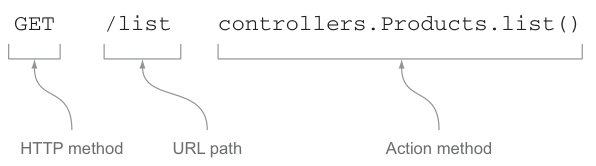
\includegraphics[scale=0.8]{Gambar/2_routes.PNG}
	\caption{Struktur kode \textit{file} ``routes''\cite{playforjava}}
	\label{fig:2_routes}
\end{figure}

URL \textit{path} dan \textit{action method} pada \textit{routes} juga dapat berisi sebuah nilai variabel. Berikut adalah contoh penulisan program URL \textit{path} dan \textit{action method} pada \textit{routes} yang berisi sebuah nilai variabel:

\begin{lstlisting}
	GET   /clients/:id          controllers.Clients.show(id: Long)
\end{lstlisting}

Penulisan sebuah variabel pada URL \textit{path} dimulai dengan tanda ``:'' lalu diikuti dengan nama variabel yang diinginkan, contohnya: ``\texttt{:id}''. Ketika menggunakan variabel pada URL \textit{path}, pada \textit{action method} perlu ditambahkan deklarasi variabel yang diletakan di dalam bagian \textit{method} yang dipilih. Cara penulisan deklarasi variabel pada \textit{action method} adalah dimulai dengan nama variabel, lalu diikuti karakter ``:'', dan diakhiri dengan tipe variabel yang diinginkan. Contoh penulisan deklarasi variabel di dalam \textit{method} suatu kelas pada bagian \textit{action method} adalah ``\texttt{id: Long}''. 

\textbf{\textit{Models}}

Fungsi \textit{models} pada Play Framework sama seperti fungsi \textit{models} pada pola arsitektur MVC secara umum, yaitu untuk memanipulasi dan menyimpan data. Secara \textit{default}, \textit{models} tidak dibuat oleh struktur minimal Play Framework (gambar \ref{fig:2_strukturplay}). Untuk itu perlu menambahkan \textit{models} secara manual ke dalam struktur Play Framework. Langkah yang dilakukan untuk menambahkan \textit{models} ke dalam Play Framework adalah:
\begin{enumerate}
	\item Menambahkan folder ``models'' ke dalam folder ``app'',
	\item Menambahkan file dengan format ``.java'' ke dalam folder ``models''.
\end{enumerate}

Tidak ada aturan khusus yang diharuskan dalam penulisan kode dalam kelas \textit{models}. Selama kelas \textit{models} yang dibuat memenuhi aturan bahasa Java, maka \textit{models} dapat dieksekusi oleh \textit{server} Play Framework.

\textbf{\textit{Views}}

Fungsi \textit{views} pada Play Framework adalah mengatur tampilan yang ingin ditampilkan di layar. \textit{Views} menggunakan bahasa HTML dan Scala. Bahasa Scala pada \textit{views} berfungsi sebagai penerima parameter yang dikirimkan dari kelas \textit{models} dimana antara \textit{models} dan \textit{views} dihubungkan oleh \textit{controllers}. Penamaan \textit{file} di dalam folder \textit{views} (gambar \ref{fig:2_strukturplay}) harus dengan format sebagai berikut, ``namaFile.scala.html''.

Berikut adalah contoh struktur kode \textit{views}:

\begin{lstlisting}
@(name:String)
<!doctype html>
<html>
	<head>
		<meta charset="UTF-8">
		<title>Hello</title>
	</head>
	<body>
		<h1>Hello <em>@name</em></h1>
	</body>
</html>
\end{lstlisting}

Baris 1 pada contoh kode di atas digunakan sebagai parameter penerima input dari \textit{models} yang dihubungkan dengan \textit{controllers}. Format deklarasi variabel pada parameter \textit{views} diawali dengan karakter ``@'', lalu diikuti dengan ``(namaVariabel$_1$: tipeVariabel$_1$) (namaVariabel$_2$: tipeVariabel$_2$) \ldots (namaVariabel$_n$: tipeVariabel$_n$)'', dimana n adalah jumlah parameter yang ingin digunakan dalam \textit{views}. Variabel pada parameter yang sudah dideklarasikan dapat dipanggil dengan menggunakan format ``@namaVariabel'' (baris 9).

\textbf{\textit{Controllers}}

\textit{Controllers} merupakan bagian pada Play Framework yang terhubung langsung dengan \textit{routes}. Jika \textit{action method} yang dikirimkan oleh \textit{routes} sesuai dengan \textit{method} yang dimiliki suatu kelas \textit{controllers}, maka \textit{controllers} akan mengeksekusi fungsi logika yang terdapat pada \textit{method} dan mengembalikan nilai berupa objek dari kelas \textit{Result} (gambar \ref{fig:2_controllers1}). Fungsi dari \textit{controllers} dalam arsitektur MVC adalah sebagai penghubung antara \textit{models} dan \textit{views}. 

\begin{figure}[htbp]
	\centering	
		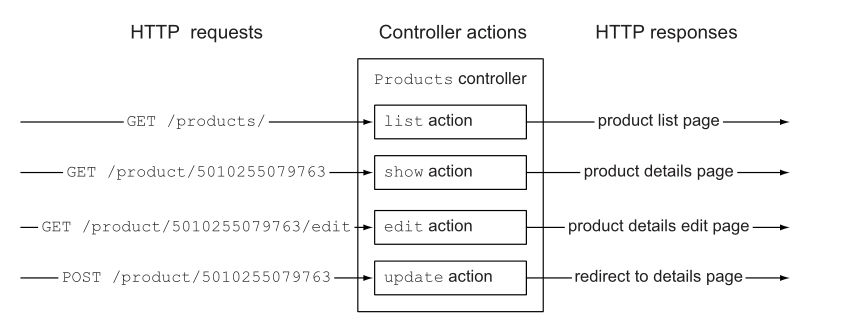
\includegraphics[scale=0.7]{Gambar/2_controllers1.PNG}
	\caption{Hubungan \textit{routes} dan \textit{controllers} dalam memproses HTTP \textit{requests}\cite{playforjava}}
	\label{fig:2_controllers1}
\end{figure}

Berikut adalah contoh penulisan program suatu kelas \textit{controllers}:

\begin{lstlisting}
package controllers;

import play.mvc.Controller;

public class Application extends Controller {

	public Result index() {
		return ok(index.render("Your new application is ready."));
	}

}
\end{lstlisting}

Penulisan kode pada suatu kelas \textit{controllers} menggunakan bahasa Java dan memiliki aturan khusus (contoh kode di atas). Aturan khusus dijelaskan ke dalam poin-poin sebagai berikut:
\begin{enumerate}
	\item \textit{Visibility} kelas dan \textit{method} pada kelas tersebut harus \textit{public} (baris 5),
	\item Kelas yang dibuat harus merupakan turunan dari ``\texttt{play.mvc.Controller}'' (baris 5),
	\item Nilai kembalian \textit{method} yang dibuat dalam suatu kelas \textit{controllers} harus berupa objek dari kelas Result (baris 7 dan 8).
\end{enumerate}
	
\textbf{\textit{Database}}

Play Framework menyediakan sebuah \textit{plugin} yang dapat digunakan untuk mengatur koneksi JDBC ke berbagai jenis aplikasi \textit{database} yang tersedia\cite{playframeworkweb}. Salah satu koneksi \textit{database} yang disediakan oleh Play adalah koneksi ke MySQL. Secara \textit{default} \textit{plugin} yang disediakan oleh Play masih belum aktif. Perlu dilakukan beberapa langkah agar \textit{plugin} tersebut dapat aktif. Berikut adalah langkah-langkah yang dilakukan agar Play Framework dapat terhubung dengan \textit{database} MySQL:
\begin{enumerate}
	\item Menambahkan kode program ke dalam ``build.sbt'' (gambar \ref{fig:2_strukturplay}), yaitu:
	
	\begin{lstlisting}
	libraryDependencies += javaJdbc
	libraryDependencies += "mysql" % "mysql-connector-java" % "5.1.18"
	\end{lstlisting}
	
	Baris 1 kode program di atas adalah untuk mengaktifkan plugin JDBC pada Play Framework. Play tidak menyediakan \textit{database driver} apapun, untuk itu perlu menambahkan \textit{database driver} (baris 2) sebagai \textit{dependency} untuk aplikasi Play Framework.
	
	\item Menambahkan kode program ke dalam ``conf/application.conf'' (gambar \ref{fig:2_strukturplay}), yaitu:
	
	\begin{lstlisting}
	db.default.driver=com.mysql.jdbc.Driver
	db.default.url="jdbc:mysql://localhost/playdb"
	db.default.username=playdbuser
	db.default.password="a strong password"
	\end{lstlisting}
	
	Baris 1 kode program di atas menyatakan jenis \textit{driver} yang digunakan, yaitu MySQL. Baris 2 kode program menyatakan nama database yang digunakan, yaitu ``playdb''. Baris 3 dan 4 menyatakan \textit{username} dan \textit{password} yang dibutuhkan dalam otentikasi terhadap \textit{server database} untuk mendapatkan hak akses tertentu terhadap \textit{database}.
\end{enumerate}

	Salah satu aktivitas programming yang dibantu JDBC adalah menghubungkan aplikasi Java ke suatu sumber data seperti \textit{database}. Play Framework telah menyediakan kelas ``DB'' yang dapat memudahkan aplikasi Java membuat suatu koneksi dengan \textit{database}. Berikut adalah contoh kode yang diperlukan untuk menggunakan kelas ``DB'' dari Play Framework:
	\begin{lstlisting}
	import play.db.*;

	Connection connection = DB.getConnection();
	\end{lstlisting}
	Contoh kode di atas menyederhanakan penulisan kode milik JDBC. 
	
\item \textbf{JSON}

JSON (\textit{JavaScript Object Notation}) adalah sebuah format pertukaran data ringan\cite{json}. JSON dapat dibangun dalam 2 buah struktur:
\begin{enumerate}
	\item Sekumpulan pasangan antara nama dengan nilai. Umumnya dikenal dengan sebutan objek. Sebuah objek dalam JSON dimulai dengan karakter ``\texttt{\{}'' dan diakhiri dengan karakter ``\texttt{\}}''. Diantara karkater ``\texttt{\{}'' dan ``\texttt{\}}'' dapat disisipkan sekumpulan pasangan ``\texttt{nama:nilai}'' yang dipisahkan dengan karakter ``\texttt{,}''.
	\item Sekumpulan data terstruktur. Umumnya dikenal dengan sebutan \textit{array}. Sebuah \textit{array} dalam JSON dimulai dengan karakter ``\texttt{[}'' dan diakhiri dengan karakter ``\texttt{]}''. Diantara karkater ``\texttt{[}'' dan ``\texttt{]}'' dapat disisipkan sekumpulan data (dapat berupa nilai, objek atau \textit{array}) yang dipisahkan dengan karakter ``\texttt{,}''. Dalam \textit{array}. Setiap data dalam \textit{array} tidak harus sama jenisnya.
\end{enumerate}

Nilai dalam JSON dapat berupa \textit{string} (sekumpulan karakter yang diapit dengan 2 tanda kutip ganda, contoh: ``\texttt{karakter}''), angka, \texttt{true}, \texttt{false}, atau \texttt{null}.

Berikut adalah contoh sebuah data JSON:
\begin{lstlisting}
	{
		"status":"error",
		"message":"Value of userid is expected but not found"
	}
\end{lstlisting}

Contoh kode di atas adalah sebuah objek (baris 1-4) yang memiliki 2 buah pasangan ``\texttt{nama:nilai}'' yang dipisahkan oleh karakter ``\texttt{,}'' (baris 2-3). Contoh di atas juga menggunakan \textit{string} sebagai nilainya (baris 2 dan 3).


		\end{itemize}

		\item Menganalisis teori-teori untuk membangun KIRI \textit{Dashboard Server Side} dalam bahasa Java dengan menggunakan Play Framework.\\
		{\bf status :} Ada sejak rencana kerja skripsi.\\
		{\bf hasil :} Mengerti penggunaan \textit{controllers}, \textit{routes}, dan \textit{views} (sedikit). Mencoba membuat kode untuk fungsi CRUD (masih gagal).

		\item Merancang KIRI \textit{Dashboard Server Side} dalam bahasa Java dengan menggunakan Play Framework.\\
		{\bf status :} Ada sejak rencana kerja skripsi.\\
		{\bf hasil :} belum ada perkembangan.

		\item Melakukan \textit{porting} kode situs web KIRI \textit{Dashboard Server Side} yang semula dalam bahasa PHP menjadi bahasa Java dengan menggunakan Play Framework.\\
		{\bf status :} Ada sejak rencana kerja skripsi.\\
		{\bf hasil :} belum ada perkembangan.
		
		\item Melakukan pengujian terhadap fitur-fitur yang sudah dibuat\\
		{\bf status :} Ada sejak rencana kerja skripsi.\\
		{\bf hasil :} belum ada perkembangan.

		\item Menulis dokumen skripsi.\\
		{\bf status :} Ada sejak rencana kerja skripsi.\\
		{\bf hasil :} Sudah menulis dokumen skripsi bab 1 dan bab 2.
	\end{enumerate}

\bibliographystyle{ieeetr}
\bibliography{pustaka}

\section{Pencapaian Rencana Kerja}
Persentase penyelesaian skripsi sampai dengan dokumen ini dibuat dapat dilihat pada tabel berikut :

\begin{center}
  \begin{tabular}{ | c | c | c | c | l | c |}
    \hline
    1*  & 2*(\%) & 3*(\%) & 4*(\%) &5* &6*(\%)\\ \hline \hline
    1   & 10 & 10 &    &  & 6 \\ \hline
    2   & 10 & 10 &    &  & 8 \\ \hline
    3   & 15 & 15 &    &  & 3 \\ \hline
    4   & 15 &    & 15 &  & 0 \\ \hline
    5   & 15 &    & 15 &  & 0 \\ \hline
    6   & 15 &    & 15 &  & 0 \\ \hline
    7   & 20 & 5  & 15 & {\footnotesize penulisan skripsi hingga bab 3 pada S1} & 3 \\ \hline
    Total  & 100  & 40  & 60 &  & 20\\ \hline
                          \end{tabular}
\end{center}

Keterangan (*)\\
1 : Bagian pengerjaan Skripsi (nomor disesuaikan dengan detail pengerjaan di bagian 5)\\
2 : Persentase total \\
3 : Persentase yang akan diselesaikan di Skripsi 1 \\
4 : Persentase yang akan diselesaikan di Skripsi 2 \\
5 : Penjelasan singkat apa yang dilakukan di S1 (Skripsi 1) atau S2 (skripsi 2)\\
6 : Persentase yang sidah diselesaikan sampai saat ini 

\vspace{1cm}
\centering Bandung, \tanggal\\
\vspace{2cm} \nama \\ 
\vspace{1cm}

Menyetujui, \\
\ifdefstring{\jumpemb}{2}{
\vspace{1.5cm}
\begin{centering} Menyetujui,\\ \end{centering} \vspace{0.75cm}
\begin{minipage}[b]{0.45\linewidth}
% \centering Bandung, \makebox[0.5cm]{\hrulefill}/\makebox[0.5cm]{\hrulefill}/2013 \\
\vspace{2cm} Nama: \pembA \\ Pembimbing Utama
\end{minipage} \hspace{0.5cm}
\begin{minipage}[b]{0.45\linewidth}
% \centering Bandung, \makebox[0.5cm]{\hrulefill}/\makebox[0.5cm]{\hrulefill}/2013\\
\vspace{2cm} Nama: \pemB \\ Pembimbing Pendamping
\end{minipage}
\vspace{0.5cm}
}{
% \centering Bandung, \makebox[0.5cm]{\hrulefill}/\makebox[0.5cm]{\hrulefill}/2013\\
\vspace{2cm} Nama: \pembA \\ Pembimbing Tunggal
}
\end{document}

